\documentclass[12pt, spanish, pdftex]{UC3M_document}

%%%%% Preamble %%%%%
\author{Jorge Rodríguez Fraile}
\authorstwotrue
\authorsuptothree{Jorge Rodríguez Fraile}{100405951}{Grupo 83}{}{}{}{}{}{}


%%%%% Basic data about the document (Degree, subject, title, campus, page number custom text) %%%%%
\documentdata{Grado en Ingeniería Informática}{Algoritmos Genéticos y Evolutivos}{Práctica 2 \\ Calibración de motores automática mediante Estrategias Evolutivas}{Leganés}{}

%%%%% Page style %%%%%
\header
\footer
\pagestyle{fancy}

\begin{document}
%%%%% Page title %%%%%
\begin{titlepage}
	\centeredtitle{img/LogoUC3M.png}{\studyname}{Curso 2021-2022}{\subjectname}{\documenttitle}
	
	\begin{table}[b]
		\centering
		\begin{tabular}{ cccc }
			\large Jorge Rodríguez Fraile & \large 100405951 & \large Grupo 83 & \href{mailto:100405951@alumnos.uc3m.es}{\large 100405951@alumnos.uc3m.es} \\
			                              &                  &                 &                                                                           \\
			                              &                  &                 &                                                                           \\
		\end{tabular}
	\end{table}
	
\end{titlepage}

\newpage

%%%%% Index %%%%%
\begin{spacing}{0.5}
	% \shipout\null                   % Blank page before index (after title page)
	\hypersetup{linkcolor=black}    % References/links on the index will remain black color
	\tableofcontents\newpage        % Index of the document
	\listoffigures\newpage          % Index of pictures
	\listoftables\newpage           % Index of tables
\end{spacing}


%%%%% DOCUMENT CONTENT %%%%%
\section{Introducción}
Este proyecto trata sobre encontrar una aproximación mediante estrategias evolutivas al problema de calibrar motores de un brazo robótico utilizando solo un láser, una cámara y un objeto de referencia. El robot deberá ser preciso en sus movimientos, dado que será utilizado para realizar soldaduras de alta precisión.

Para comenzar se trabajará sobre un brazo compuesto solo por 4 motores para podernos acercar al problema de una manera más gradual, en cuanto se haya comprobado que es factible esta simplificación del problema se pasara a un caso más realista con un brazo de 10 motores.

\section{Codificación y Función de fitness}
Al emplear estrategias evolutivas la codificación de los individuos de este problema consistirá en un vector de codificación compuesto por 4 o 10 números reales (según el número de motores) y un vector de varianzas de la misma longitud que el de codificación.

Los valores del vector de codificación estarán centrados en 0 representando que no se ha realizado ningún giro y podrán rotar tanto como quieran en sentido positivo como negativo, aunque llegado un punto girar mucho en un sentido equivale a movimientos más cortos. Lo ideal es que los valores se muevan entre -180 y 180 grados representando un giro completo de 360 grados, aunque no se restringirán los valores que puede tomar. En la \autoref{fig:diagramaBrazo} se puede ver un diagrama de cómo es el sistema.
\begin{figure}[H]
	\ffigbox[\FBwidth]
	{\caption{Diagrama brazo robótico}
	\label{fig:diagramaBrazo}}
	{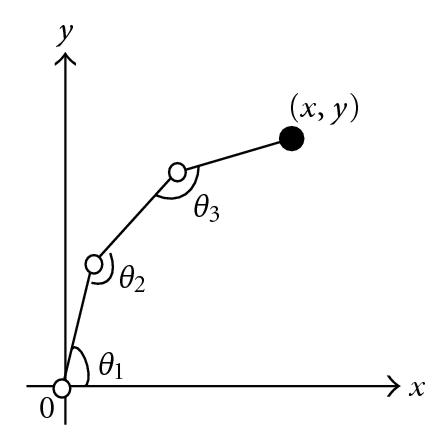
\includegraphics[scale=1.5]{./img/arm_angles.jpg}}
\end{figure}

En cuanto a la función de fitness que se empleará para saber si una solución es buena o no, esta tendrá en cuenta el error que comente el soldador en un simulador, según como de dispersos y desviados sean con respecto al centro dará un valor mayor cuanto peor lo haga y menor cuanto más preciso sea. Por lo que el objetivo del problema es minimizar la función de fitness.

Para conocer el error para cada una se las soluciones se hará una llamada get a un servicio que se encuentra en un servidor de la universidad, \href{http://memento.evannai.inf.uc3m.es/age/robot4?}{http://memento.evannai.inf.uc3m.es/age/robot4?}, seguido de cX=GradosDeX para cada uno de los 4 motores y separados por un $\&$, en el caso de los 10 motores será igual, aunque con otro servicio \href{http://memento.evannai.inf.uc3m.es/age/robot10?}{http://memento.evannai.inf.uc3m.es/age/robot10?} y 10 valores de grados.

\section{Programación Estrategia Evolutiva (1+1)}
Para este proyecto entre las posibles implementaciones de las estrategias evolutivas se ha elegido la (1+1)-EE y a continuación se describirán las características de esta. 

El programa se ha desarrollado en el lenguaje Python, el procesamiento principal del programado se encuentra en la función \textit{EE1plus1(c, cycles, test\_iteration)}, donde recibirá como parámetros el valor por el que se multiplicaran las varianzas, el número de generaciones máximas del programa y la iteración en la que se encuentra el programa (se incluye para realizar las pruebas de ejecutar múltiples veces).

El proceso que sigue esta función es el siguiente:
\begin{enumerate}
	\item Generar el individuo inicial.
	\item Evaluar el individuo generado de la población inicial.
	\item Repetir hasta cumplir el criterio de convergencia:
	      \begin{enumerate}
		      \item Generar una nueva solución a partir del único individuo de la población, mutando el vector de codificación del descendiente.
		      \item Evaluar el individuo generado.
		      \item Eliminar el individuo cuyo valor de adecuación sea mayor, tratamos de minimizar el fitness.
		      \item Si el individuo que queda es el nuevo, se aumenta la frecuencia de éxitos y si no se disminuye.
		      \item Mutar el vector de varianzas del individuo elegido de acuerdo con la regla 1/5.
	      \end{enumerate}
\end{enumerate}

Además de lo relacionado con la generación de individuos, también se ha incluido código que nos permita almacenar la salida de los modelos para poderlos evaluar.

\subsection{Operadores genéticos}
\subsubsection{Población inicial}
El individuo inicial es generado aleatoriamente, para su vector de codificación se sigue una gaussiana centrada en 0 y con desviación 100, de esta manera los valores serán tanto positivos como negativos y mayoritariamente centrados alrededor de 0, por otro lado el vector de varianzas se genera mediante valores reales positivos entre 5 y 20, aunque se realizarán pruebas con valores mayores.

Este proceso es realizado por la función \textit{initial\_individual()}, devolviendo un individuo en forma de matriz con dimensiones NumeroDeMotores x 2.  

\subsubsection{Mutación}
Para los algoritmos evolutivos este operador se realiza en dos partes una para el vector de codificación y otra para el de varianzas.

Para el vector de codificación, el nuevo individuo tendrá como valores los del progenitor más un valor de la normal según la varianza de ese valor para el padre, es decir $x_{hijo}=x_{padre}+N_0(\sigma_{padre})$, esta operación se repite para todos los valores del vector.

En cuanto al vector de varianzas, se realizará sobre el individuo seleccionado para la siguiente generación, y consiste en modificar sus varianzas en función de la regla 1/5, que se guía por el porcentaje de mejoras de las últimas generaciones. Esta regla se aplicará teniendo en cuenta las últimas generaciones, las variaciones vendrán dadas por:
\begin{itemize}
	\item Si el número de mejoras es superior al 20 \%, se aumenta la varianza $\frac \sigma c$.
	\item Si el número de mejoras es inferior al 20 \%, se reduce la varianza $\sigma \cdot c$.
	\item Si el número de mejoras es igual al 20 \%, se mantiene $\sigma$.
\end{itemize}

Lo que dice la regla es que si mejora con frecuencia es que todavía estamos lejos de la solución óptima, por lo que aumentaremos la varianza, y si no mejora es que estamos cerca, entonces nos movemos poco a poco.

Esta funcionalidad se recoge en \textit{mutate\_codification(individual)} para el vector de codificación, muta al progenitor y devuelve al sucesor, y en \textit{individual\_next\_generation(individual, son, improvements\_counter, iteration, c)} para el vector de varianzas, se encuentran separadas porque hasta que no se conoce el individuo de la siguiente generación no se mutan las varianzas.

\subsubsection{Inserción y Remplazo}
Al tratarse del tipo (1+1) la población está formada por un solo individuo y también se generará un solo individuo, por lo que entre el individuo de la población y el nuevo se elegirá el mejor, en este caso el de menor fitness.

Cuando se elija al descendiente se considera una mejora y se tendrá en cuanta en la frecuencia de mejoras, si no, se considera que no ha mejorado. Tras elegir el individuo que formará la población se mutará su vector de varianzas como se ha definido antes.

La función que recoge la inserción y remplazo, además de la mutación de las varianzas es la que se mencionó antes, \textit{individual\_next\_generation(individual, son, improvements\_counter, iteration, c)}, que evalúa ambos individuos, elige el mejor, actualiza el contador de mejoras y aplica la mutación en función del parámetro c que se le pasa. La función devuelve el individuo elegido, su fitness y el contador de mejoras actualizado. 

\subsection{Aproximación 4 motores}\label{sec:4m}
Comenzaremos realizando pruebas en la versión simplificada del problema, en el que solo se consideraran 4 motores para el brazo soldador. 

Estos primeros modelos que se generaran consistirán en la variación del valor c, el que determina cuanto cambiara la varianza de los individuos. Es conocido que el valor debe ser inferior a 1 y que el recomendable es 0,82, pero en busca de mejores resultados se ha probado además con 0,98, 0,92, 0,72 y 0,62. No se han variado más estos valores, porque la selección de valores más bajos provocaría que los valores de varianza se movieran muy rápido.

Todos los modelos se han ejecutado durante 5000 generaciones, que son 10000 evaluaciones, y se han realizado 10 ejecuciones para cada modelo para evitar el sesgo de la aleatoriedad a la hora de inicializar el modelo.

Los modelos han sido nombrados siguiendo el siguiente patrón: evolution\_strategy\_XX\_YY\_A-B\_C
\begin{itemize}
	\item \textbf{XX:} Indica el número de motores que se consideran y para los que se ajustaran los ángulos.
	\item \textbf{YY:} Indica el valor de c, el cual determina como se modificarán las varianzas.
	\item \textbf{A-B:} Indica el rango de valores entre los que se generan aleatoriamente las varianzas.
	\item \textbf{C:} Indica el número de generaciones que tiene en cuanta para medir la frecuencia de mejora.
\end{itemize}

En la \autoref{fig:fitness4inicial} y \autoref{tab:fitness4inicial} se pueden ver los resultados de fitness obtenidos en las \textbf{10 ejecuciones para los 5 modelos}, junto a la media de cada modelo que es la que utilizaremos para comparar.
\begin{figure}[H]
	\ffigbox[\FBwidth]
	{\caption{Valores de Fitness: 4\_5-20\_10}
	\label{fig:fitness4inicial}}
	{\includegraphics[scale=.6]{./img/Fitness\_4\_5-20\_10.png}}
\end{figure}
\begin{table}[H]
	\centering
	\resizebox{\textwidth}{!}{%
		\begin{tabular}{|c|c|c|c|c|c|c|c|c|c|c|c|}
			\hline
			\rowcolor[HTML]{BFBFBF}
			\textbf{Modelo}                                    & \textbf{1}  & \textbf{2}  & \textbf{3}  & \textbf{4}  & \textbf{5}  & \textbf{6}           & \textbf{7}  & \textbf{8}  & \textbf{9}  & \textbf{10} & \textbf{Media}       \\ \hline
			\cellcolor[HTML]{BFBFBF}\textbf{4\_0,98\_5-20\_10} & 399,8967664 & 21,88903367 & 20,89403404 & 1,989918114 & 2,984877171 & \textbf{0,994959057} & 243,1577278 & 13,92939149 & 49,74695184 & 5,969749305 & \textbf{76,14534088} \\ \hline
			\cellcolor[HTML]{BFBFBF}\textbf{4\_0,92\_5-20\_10} & 115,4108682 & 86,56039686 & 587,9440061 & 654,4753316 & 51,73723573 & 25,86868199          & 35,81824234 & 125,3603064 & 2081,267141 & 4,974790248 & 376,9417             \\ \hline
			\cellcolor[HTML]{BFBFBF}\textbf{4\_0,82\_5-20\_10} & 34,8234203  & 1053,037537 & 98,49807057 & 263,6453657 & 79,59564625 & 270,6192328          & 1955,329393 & 1649,132003 & 193,0126789 & 361,1448922 & 595,8838239          \\ \hline
			\cellcolor[HTML]{BFBFBF}\textbf{4\_0,72\_5-20\_10} & 134,6082641 & 887,2371193 & 758,3690516 & 1232,534402 & 731,1155627 & 161,1833393          & 208,9351831 & 808,6563643 & 1438,833559 & 993,6769101 & 735,5149756          \\ \hline
			\cellcolor[HTML]{BFBFBF}\textbf{4\_0,62\_5-20\_10} & 1342,19067  & 58,71220968 & 24,87415781 & 1391,691525 & 1691,348176 & 1280,418402          & 443,7601042 & 692,0338572 & 1812,167475 & 113,4223726 & 885,061895           \\ \hline
		\end{tabular}%
	}
	\caption{Fitness iniciales 4 motores}
	\label{tab:fitness4inicial}
\end{table}

Se puede ver que los mejores resultados se han obtenido para una c de 0,98 y que según se van reduciendo progresivamente, las evaluaciones van empeorando. En la \autoref{fig:fitness4inicial} solo se ve el valor para la media, pero en la \autoref{tab:fitness4inicial} se puede apreciar que los valores normalmente son bajos y los que la suben son unas pocas ejecuciones que dan valores más altos. 

Aun con esto, el mejor resultado se ha obtenido en la que da mejor media, que es \textbf{c de 0,98} y una ventana de \textbf{varianzas entre 5 y 20}. El resultado que nos proporciona el modelo es de \textbf{0,994959057 de fitness}, que le lleva \textbf{1998 evaluaciones}, que para el caso son 999 generaciones de las 5000 dadas. 

\textbf{De media este modelo requiere 2670 evaluaciones} para alcanzar su mejor resultado, que es \textbf{de media 76,14534088 de fitness}.

En la siguiente página se puede ver en la \autoref{fig:mejor4mEval} el progreso del fitness y en la \autoref{fig:mejor4mAng} el de los ángulos a lo largo de las 1998 evaluaciones. Al comienzo como los valores de partida son aleatorios el error es muy alto y rápidamente decrece hasta converger, en este caso en torno al 1. En cuanto a los grados se aprecia un comportamiento parecido, se van moviéndose rápidamente hasta llegar a un valor en el que converge en este caso los valores son:
\begin{itemize}
	\item \textbf{Motor 1:} 9,128498158310796
	\item \textbf{Motor 2:} 5,9876539870877865 
	\item \textbf{Motor 3:} 3,6666659795960044 
	\item \textbf{Motor 4:} 1,7654321185803394
\end{itemize}
\begin{figure}[H]
	\ffigbox[\FBwidth]
	{\caption{Fitness vs. Evaluaciones: 4\_5000\_0.98\_6}
	\label{fig:mejor4mEval}}
	{\includegraphics[scale=.6]{./img/4\_5000\_0.98\_6Eval.png}}
\end{figure}
\begin{figure}[H]
	\ffigbox[\FBwidth]
	{\caption{Ángulos: 4\_5000\_0.98\_6}
	\label{fig:mejor4mAng}}
	{\includegraphics[scale=.6]{./img/4\_5000\_0.98\_6Ang.png}}
\end{figure}

Después de ver esto, pasamos a probar aumentando el número de generaciones que se tienen en cuenta para la regla 1/5, pasaremos de 10 generaciones a 100, de esta manera se intentará suavizar un poco que pase de aumentar a reducir las varianzas. Se repiten de nuevo las pruebas anteriores para ver si este cambio supone una mejora en  general en los modelos que se habían considerado.

Los resultados que obtenemos durante \textbf{10 ejecuciones para 4 motores, c variable y teniendo en cuenta 100 generaciones} para las varianzas se describen en la \autoref{fig:4mFitness2} y la \autoref{tab:4mFitness2}.

\begin{figure}[H]
	\ffigbox[\FBwidth]
	{\caption{Valores de Fitness: 4\_5-20\_100}
	\label{fig:4mFitness2}}
	{\includegraphics[scale=.58]{./img/Fitness\_4\_5-20\_100.png}}
\end{figure}
\begin{table}[H]
	\centering
	\resizebox{\textwidth}{!}{%
	\begin{tabular}{|c|c|c|c|c|c|c|c|c|c|c|c|}
	\hline
	\rowcolor[HTML]{BFBFBF} 
	\textbf{Modelo}                                     & \textbf{1}  & \textbf{2}  & \textbf{3}  & \textbf{4}  & \textbf{5}  & \textbf{6}           & \textbf{7}           & \textbf{8}  & \textbf{9}  & \textbf{10} & \textbf{Media}       \\ \hline
	\cellcolor[HTML]{BFBFBF}\textbf{4\_0,98\_5-20\_100} & 5,969749305 & 21,8889931  & 9,949580495 & 4,974790248 & 5,969749305 & 5,969749305 & \textbf{1,989918114} & 6,964708362 & 2,984877171 & 3,979836228 & \textbf{7,064195163} \\ \hline
	\cellcolor[HTML]{BFBFBF}\textbf{4\_0,92\_5-20\_100} & 5,542532418 & 14,74571547 & 84,98910986 & 37,81101029 & 5,011906134 & 36,82614644          & 34,11110903          & 10,47056077 & 53,73206948 & 27,85876286 & 31,10989227          \\ \hline
	\cellcolor[HTML]{BFBFBF}\textbf{4\_0,82\_5-20\_100} & 9,809572078 & 41,36192181 & 99,24012352 & 339,3468103 & 42,84572441 & 36,74907856          & 18,86484429          & 30,76219558 & 20,6740378  & 28,65534023 & 66,83096486          \\ \hline
	\cellcolor[HTML]{BFBFBF}\textbf{4\_0,72\_5-20\_100} & 263,4369112 & 67,53778001 & 119,6652832 & 29,2806866  & 22,87188578 & 107,3685088          & 277,6832855          & 27,53812501 & 187,4785023 & 103,624326  & 120,6485294          \\ \hline
	\cellcolor[HTML]{BFBFBF}\textbf{4\_0,62\_5-20\_100} & 67,02456414 & 60,89633218 & 280,0429631 & 63,05976061 & 42,89979308 & 28,0932833           & 76,75306751          & 478,2493174 & 43,57174374 & 34,51221151 & 117,5103037          \\ \hline
	\end{tabular}%
	}
	\caption{Fitness 4 motores y 100 generaciones modificar varianzas}
	\label{tab:4mFitness2}
	\end{table}

Se puede ver que los modelos mantienen la misma distribución que en la experimentación previa, es decir que los resultados son mejores cuanto mayor es el c, pero en este caso se reducen en general los valores de fitness.

La media del \textbf{fitness es 10 veces más pequeño} que su equivalente de la prueba anterior y esto se repite de la misma manera para los otros modelos. El mejor modelo en este caso tiene de \textbf{media 7,064195163 de fitness}.

Aunque de manera general se han reducido las evaluaciones, el mejor resultado obtenido no es mejor que el previo.

El mejor resultado se sigue correspondiendo con una \textbf{c de 0,98 valores de varianza iniciales entre 5 y 20}, pero en esta prueba en particular se han tenido en cuenta \textbf{100 generaciones para la regla 1/5}. El valor de \textbf{fitness de este modelo es 1,989918114}, que lo alcanza \textbf{en la evaluación 1990}, al igual que el otro esta evaluación está lejos del límite máximo de evaluaciones y le ha dado tiempo a converger correctamente. De media el mejor resultado para este modelo se obtiene en la evaluación 1962. Esta solución se corresponde con:
\begin{itemize}
	\item \textbf{Motor 1:} 1,98991811419
	\item \textbf{Motor 2:} 9,128498154683596 
	\item \textbf{Motor 3:} 4,99269532895493
	\item \textbf{Motor 4:} 1,7654320755166042
\end{itemize}
\pagebreak

Con estas dos pruebas se ha podido ver que este método es factible para el problema y alcanza valores realmente buenos, cercanos al 0. En cuanto a la cantidad de generaciones que considerar para modificar las varianzas parecen mejor 100, pero en ejecuciones puntuales 10 también es buena, por lo que en la siguiente sección con 10 motores se repetirán los experimentos para ver si se puede concluir lo mismo.

\subsection{Aproximación 10 motores}\label{sec:10m}
Tras haber realizado unas pruebas iniciales con una versión simplificada para ver que es factible emplear esta técnica al problema pasamos al problema real, un brazo robótico de soldadura de 10 motores o articulaciones que se mueven de manera independiente y con el que tendremos que tratar de alcanzar la mejor configuración para que sea preciso.

Se volverá a probar con \textbf{5 valores de c (0,98, 0,92, 0,72 y 0,62)} como se hizo en la sección anterior, pero en este caso como se van a configurar \textbf{10 motores} se le dejaran \textbf{10000 generaciones, 20000 evaluaciones}, para que el de tiempo a converger y se haya obtenido el mejor resultado de la ejecución.

A continuación en la \autoref{fig:10mFitness1} se muestran los resultados de \textbf{10 ejecuciones teniendo en cuenta las 10 generaciones previas} para modificar las varianzas, además de la \autoref{tab:10mFitness1} con sus correspondientes valores para poder consultar mejor las ejecuciones individualmente:

\begin{figure}[H]
	\ffigbox[\FBwidth]
	{\caption{Valores de Fitness: 10\_5-20\_10}
	\label{fig:10mFitness1}}
	{\includegraphics[scale=.58]{./img/Fitness\_10\_5-20\_10.png}}
\end{figure}
\begin{table}[H]
	\centering
	\caption{Fitness 10 motores, varianzas 5-20 y c considerando 10 generaciones}
	\label{tab:10mFitness1}
	\resizebox{\textwidth}{!}{%
	\begin{tabular}{|c|c|c|c|c|c|c|c|c|c|c|c|}
	\hline
	\rowcolor[HTML]{BFBFBF} 
	\textbf{Modelo} & \textbf{1} & \textbf{2} & \textbf{3} & \textbf{4} & \textbf{5} & \textbf{6} & \textbf{7} & \textbf{8} & \textbf{9} & \textbf{10} & \textbf{Media} \\ \hline
	\cellcolor[HTML]{BFBFBF}\textbf{10\_0,98\_5-20\_10} & 80,59085566 & 54,72242403 & 122,3772289 & 88,55070259 & 126,3554685 & 124,3677632 & 82,57983737 & 162,1761055 & \textbf{31,83857359} & 75,61582174 & \textbf{94,91747811} \\ \hline
	\cellcolor[HTML]{BFBFBF}\textbf{10\_0,92\_5-20\_10} & 493,4360219 & 89,54541129 & 318,3774674 & 368,0959481 & 990,6158079 & 562,034782 & 366,1135179 & 226,8463152 & 358,1536415 & 335,2929881 & 410,8511901 \\ \hline
	\cellcolor[HTML]{BFBFBF}\textbf{10\_0,82\_5-20\_10} & 90,54006087 & 286,540584 & 179,0891408 & 105,4647007 & 235,7979006 & 199,9825131 & 183,0700586 & 767,0202184 & 498,4540123 & 879,2901677 & 342,5249357 \\ \hline
	\cellcolor[HTML]{BFBFBF}\textbf{10\_0,72\_5-20\_10} & 196,5927933 & 637,7053161 & 249,7252972 & 153,2220596 & 264,6538342 & 181,0785194 & 425,8250794 & 749,1551409 & 239,7793379 & 436,7709423 & 353,450832 \\ \hline
	\cellcolor[HTML]{BFBFBF}\textbf{10\_0,62\_5-20\_10} & 310,4180872 & 335,2775147 & 362,1496302 & 604,8171685 & 164,1662712 & 293,4897782 & 416,866646 & 417,8427783 & 725,2770965 & 550,1775361 & 418,0482507 \\ \hline
	\end{tabular}%
	}
	\end{table}

Se puede ver que aun aumentando el número de motores a 10, la distribución de resultados sigue siendo parecida, con la excepción del modelo con c de 0,92, que este caso ha empeorado siendo peor que el modelo de 0,82 y 0,72. Se profundizará en la sección \docref{sec:resultado} más en estos modelos.

Además, los fitness del \textbf{mejor modelo de esta prueba, 10\_0,98\_5-20\_10, son bastante consistentes} entre ejecuciones. En la \autoref{fig:10mCiclos1} se observa que el número de evaluaciones que requiere cada modelo para alcanzar su mejor resultado son bastante parecidos, lo que nos permite ver que todos convergen igual de rápido, pero no en los mejores resultados.

\begin{figure}[H]
	\ffigbox[\FBwidth]
	{\caption{Ciclos hasta mejor resultado: 10\_5-20\_10}
	\label{fig:10mCiclos1}}
	{\includegraphics[scale=.58]{./img/Cycles\_10\_5-20\_10.png}}
\end{figure}

Ahora pasamos a probar si \textbf{aumentando el número de generaciones a considerar para modificar las varianzas} mejoran los resultados como ocurría en el caso de los 4 motores.

\begin{figure}[H]
	\ffigbox[\FBwidth]
	{\caption{Valores de Fitness: 10\_5-20\_100}}
	{\includegraphics[scale=.58]{./img/Fitness\_10\_5-20\_100.png}}
\end{figure}
\begin{table}[H]
	\centering
	\caption{Fitness 10 motores, varianzas 5-20 y c considerando 100 generaciones}
	\resizebox{\textwidth}{!}{%
	\begin{tabular}{|c|c|c|c|c|c|c|c|c|c|c|c|}
		\hline
		\rowcolor[HTML]{BFBFBF} 
		\textbf{Modelo} & \textbf{1} & \textbf{2} & \textbf{3} & \textbf{4} & \textbf{5} & \textbf{6} & \textbf{7} & \textbf{8} & \textbf{9} & \textbf{10} & \textbf{Media} \\ \hline
		\cellcolor[HTML]{BFBFBF}\textbf{10\_0,98\_5-20\_100} & 50,74259284 & 81,58612136 & 213,9061234 & 77,60612079 & 197,9927287 & 196,9949114 & 113,4239113 & \textbf{41,78817447} & 57,08071544 & 90,54067699 & \textbf{112,1662077} \\ \hline
		\cellcolor[HTML]{BFBFBF}\textbf{10\_0,92\_5-20\_100} & 418,851877 & 245,7473547 & 255,6940882 & 222,8678002 & 143,2442372 & 733,1081525 & 284,5502886 & 373,0604005 & 212,9140302 & 380,0423028 & 327,0080532 \\ \hline
		\cellcolor[HTML]{BFBFBF}\textbf{10\_0,82\_5-20\_100} & 85,56587251 & 141,282387 & 129,4266779 & 261,6562212 & 275,588287 & 196,9962121 & 264,6484531 & 78,60131111 & 91,53563694 & 307,4233739 & 183,2724433 \\ \hline
		\cellcolor[HTML]{BFBFBF}\textbf{10\_0,72\_5-20\_100} & 134,3723279 & 148,3272106 & 240,7722142 & 80,59637497 & 153,2277586 & 362,1933594 & 122,4410243 & 263,7641307 & 180,1514111 & 347,3048804 & 203,3150692 \\ \hline
		\cellcolor[HTML]{BFBFBF}\textbf{10\_0,62\_5-20\_100} & 284,001316 & 238,3567998 & 123,5151397 & 231,8477615 & 504,8815338 & 289,2721911 & 621,3900092 & 767,7025742 & 275,3068091 & 545,6359119 & 388,1910046 \\ \hline
		\end{tabular}%
		}
		\end{table}

Como se esperaba, en general \textbf{los resultados han mejorado} con respecto a la prueba anterior, con excepción del modelo de c 0,98 que ha empeorado ligeramente. Además, mantiene la distribución de la prueba previa, siendo mejores cuanto mayor c y empeorando en c 0,92.

Nuestro mejor modelo previo era el de c 0,98 con una media de 94,91747811 de fitness y en este nuevo caso es también el de \textbf{c 0,98 con una media de 112,1662077 de fitness}. Aparte de obtener mayor fitness, el nuevo modelo \textbf{requiere 3278 evaluaciones de media} para alcanzar el mejor resultado y el otro 3186 evaluaciones.

Hasta este punto se puede concluir que los \textbf{mejores modelos se obtienen con una c de 0,98 o 0,82 y considerando 10 generaciones para mutar la varianza}.
\pagebreak

Ahora se pasará a probar para estos 2 modelos mejores modelos una \textbf{ventana de varianzas de entre 5 y 100}, además se aumentará el número de \textbf{generaciones máximas a 20000} para que puedan converger adecuadamente. Los resultados que se han obtenido son mostrados en la \autoref{fig:10mFitness2} y la \autoref{tab:10mFitness2}.
\begin{figure}[H]
	\ffigbox[\FBwidth]
	{\caption{Valores de Fitness: 10\_5-20\_10}
	\label{fig:10mFitness2}}
	{\includegraphics[scale=.58]{./img/Fitness\_10\_5-100\_10.png}}
\end{figure}
\begin{table}[H]
	\centering
	\caption{Fitness 10 motores, varianzas 5-100 y c considerando 10 generaciones}
	\label{tab:10mFitness2}
	\resizebox{\textwidth}{!}{%
	\begin{tabular}{|c|c|c|c|c|c|c|c|c|c|c|c|}
	\hline
	\rowcolor[HTML]{BFBFBF} 
	\textbf{Modelo} & \textbf{1} & \textbf{2} & \textbf{3} & \textbf{4} & \textbf{5} & \textbf{6} & \textbf{7} & \textbf{8} & \textbf{9} & \textbf{10} & \textbf{Media} \\ \hline
	\cellcolor[HTML]{BFBFBF}\textbf{10\_0,98\_5-100\_10} & 736,0960491 & 1983,36103 & 577,9290908 & 69,64607244 & 236,790299 & 134,3176337 & 1273,989951 & 1787,181803 & 71,63674394 & 710,1923834 & 758,1141056 \\ \hline
	\cellcolor[HTML]{BFBFBF}\textbf{10\_0,82\_5-100\_10} & 320,620507 & 589,2224645 & 1587,550479 & \textbf{41,78811602} & 442,778636 & 784,7749207 & 108,4492238 & 150,2370648 & 293,4932953 & 2473,840677 & \textbf{679,2755384} \\ \hline
	\end{tabular}%
	}
	\end{table}

Como se puede ver, realizando esta modificación de los valores con los que se pueden inicializar las varianzas \textbf{no produce mejores modelos}. Aun no produciendo modelos mejores en una ejecución particular alcanzó un fitness de 41,7881 que no está muy lejos del mejor modelo para los 10 motores, 31,8385.

Con todo esto se pasa a describir el mejor modelo que se ha obtenido.

\subsection{Resultado}\label{sec:resultado}
Tras todas las pruebas que se han realizado en las secciones \docref{sec:10m} y \docref{sec:4m}, se describirá en esta sección cuál es el mejor modelo que se ha obtenido para resolver el problema de hallar los ángulos para un brazo soldador de 10 motores.

El modelo que mejores fitness de media nos ha proporcionado y de una manera bastante consistente en comparación con el resto ha sido el que tiene los siguientes parámetros:
\begin{itemize}
	\item \textbf{Motores:} 10
	\item \textbf{Valores de inicialización de las varianzas:} Entre 5 y 20
	\item \textbf{c:} 0,98
	\item \textbf{Generaciones consideradas:} 10
\end{itemize}
El \textbf{fitness medio ha sido de 94,91747811}, que se ha alcanzado \textbf{en 3186,2 evaluaciones de media de las 20000} que se le ha dejado ejecutando.

En la sección \docref{sec:10m} se puede ver la consistencia del fitness con la \autoref{fig:10mFitness1} y la del número de evaluaciones en la \autoref{fig:10mCiclos1}.

\pagebreak

Analizaremos ahora la mejor ejecución de este modelo, que se corresponde con la novena ejecución y que nos proporciona los siguientes ángulos para el brazo del robot:
\begin{itemize}
	\item \textbf{Motor 1:} 2,2284984784501773
	\item \textbf{Motor 2:} 5,477566084188264
	\item \textbf{Motor 3:} 1,3246628300371095
	\item \textbf{Motor 4:} -0,22448014101449237
	\item \textbf{Motor 5:} 1,4274017184920664
	\item \textbf{Motor 6:} -3,9797837284309523
	\item \textbf{Motor 8:} -0,6517585124073262
	\item \textbf{Motor 7:} -1,055368413073764 
	\item \textbf{Motor 9:} -0,7604292115674011
	\item \textbf{Motor 10:} 3,938239892255979
\end{itemize}

Esta secuencia de ángulos nos da un \textbf{fitness de 31,83857359} que se alcanza en \textbf{3180 evaluaciones}, que equivalen a 1590 generaciones de las 10000 que se dejaron. 

En la \autoref{fig:fitness_result} se puede ver la progresión del fitness desde la primera evaluación hasta que se encuentra el mejor fitness, de esta manera se evita prolongar la gráfica en exceso para el mismo valor.

\begin{figure}[H]
	\ffigbox[\FBwidth]
	{\caption{Fitness vs. Evaluaciones: 10\_0.98\_5-20\_10}
	\label{fig:fitness_result}}
	{\includegraphics[scale=.6]{./img/10\_0.98\_5-20\_10Eval.png}}
\end{figure}
\pagebreak

De la misma manera que en la \autoref{fig:fitness_result} se puede ver en la \autoref{fig:ang_result} como van convergiendo los ángulos al ajustarse y encontrar un valor cuasi-óptimo.
\begin{figure}[H]
	\ffigbox[\FBwidth]
	{\caption{Ángulos: 10\_0.98\_5-20\_10}
	\label{fig:ang_result}}
	{\includegraphics[scale=.6]{./img/10\_0.98\_5-20\_10Ang.png}}
\end{figure}

\section{Conclusiones}
En este proyecto se ha abordado el problema de ajustar los ángulos de un brazo robótico de soldadura para que alcanzara una precisión aceptable para soldadura profesional mediante estrategias evolutivas. 

Se comenzó con una aproximación reducida con 4 motores para ver como aproximarnos al problema real y ver si esta técnica era viable para este problema específico, se puedo ver que se alcanzaban valores muy buenos menores que 1 de error.

Tras comprobar que esta aproximación es buena se pasó a problema real, 10 motores, aplicando los conocimientos adquiridos de la versión reducida. Se obtuvieron resultados con más error, cosa que se esperaba dado que cuantas más articulaciones tiene un brazo más difícil es poder calibrarlo, puesto que cualquier cambio afecta a la posición global sobre todo los más alejados de la punta del solador.

Esta práctica ha servido para ver una aplicación en primera mano de las estrategias evolutivas y ver que son una técnica potente para la resolución de problemas.


\end{document}